\section{Approach} \label{approach}
    In this chapter we will have a closer look on the different components of our approach. In figure \ref{fig:pipeline} you can see an overview of our approach. As mentionend in chapter \ref{intro} our approach consists of four components. In figure \ref{fig:pipeline} there are five components, this is due to the fact that we implemented an evaluator component to evaluate our results during development. For evaluation we used the topics and the corpus from previous years of Touché (2021 and 2020).

    \begin{figure}[h]
        \centering
        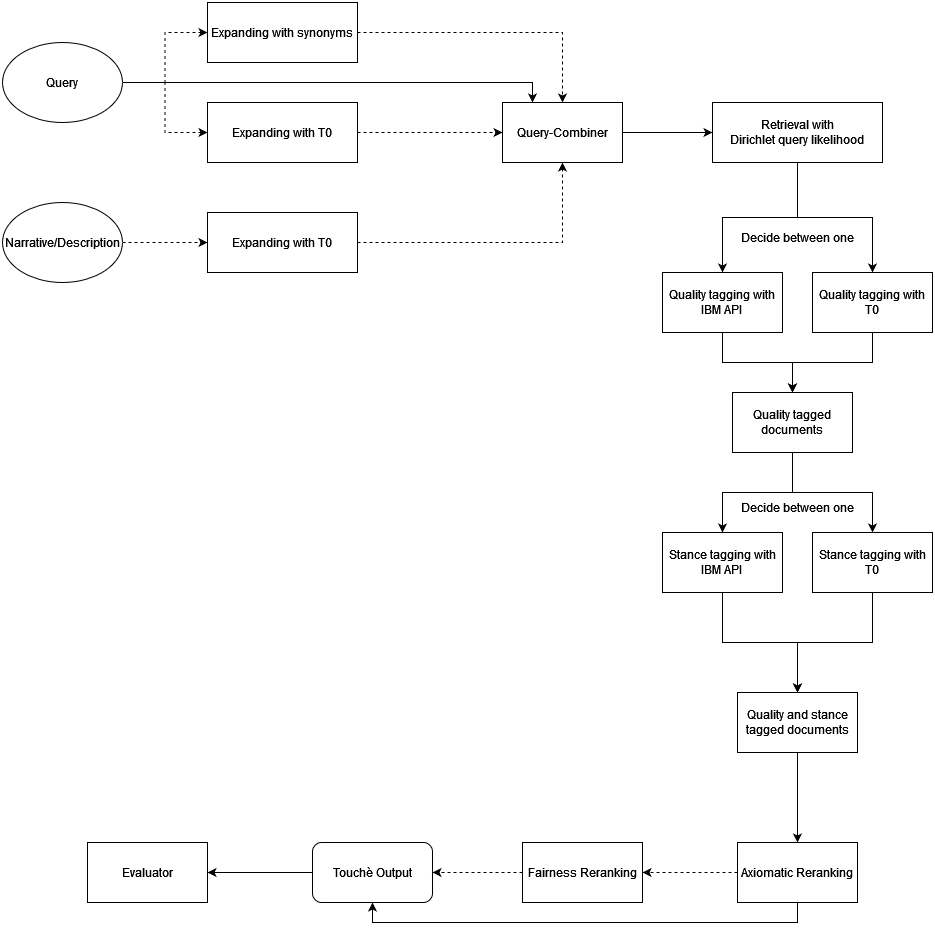
\includegraphics[scale=0.4]{figures/pipeline}
        \caption{Architecture Overview}
        \label{fig:pipeline}
    \end{figure}

    \subsection{Query Reformulation and Query Combiner}
        In this component we (a) replaced the comparative objects with synonyms and (b) used the additional information narrative and description  provided by the organizers of the shared task to generate additional queries. Using synonyms will allow us to increase the recall of our initial retrieval step by retrieving passages that contain terms similiar to the terms from the original query but would not be retrieved when using only the original query. With an higher recall we will be able to find more relevant passages which we will rerank in our last step to improve the precision of our approach. To find synonyms we used two different methods. The first method uses word embeddings and the second one uses the language model T0.    
    \subsection{Retrieval of passages}
    \subsection{Argument quality and stance tagging}
    \subsection{Axiomatic Reranker}